\chapter{Evaluation}

\section{Evaluation Methodology}
Models were evaluated using a train-test split strategy to ensure unbiased performance estimation. We focused on metrics relevant to the medical domain, specifically Recall (Sensitivity) to minimize false negatives.

\section{BO1: Tumor Classification (Diagnosis)}
This section evaluates the performance of three distinct models developed for the diagnosis task (Benign vs. Malignant): \textbf{SGD-SVM (Linear)}, \textbf{Softmax (Baseline)}, and \textbf{GRU-SVM (Hybrid)}. The evaluation prioritizes medical safety, focusing on minimizing False Negatives.

\subsection{Model Comparison Table}
The following table summarizes the key performance metrics for each model based on the final leaderboard. We specifically highlight \textbf{Sensitivity} and \textbf{False Negatives}, as these are the most critical metrics for cancer detection.

\begin{table}[H]
    \centering
    \caption{Final Leaderboard: Diagnosis Models (Test Set)}
    \begin{tabular}{lccc}
        \toprule
        \textbf{Model} & \textbf{Accuracy} & \textbf{Sensitivity} & \textbf{False Negatives} \\
        \midrule
        \textbf{SGD-SVM (Linear)} & \textbf{98.83\%} & \textbf{98.41\%} & \textbf{1} \\
        Softmax (Baseline) & 97.66\% & 96.83\% & 2 \\
        GRU-SVM (Hybrid) & 96.49\% & 96.83\% & 2 \\
        \bottomrule
    \end{tabular}
\end{table}

\subsection{Confusion Matrix Evaluation}
The confusion matrices below provide a detailed breakdown of the predictions.

\begin{figure}[H]
    \centering
    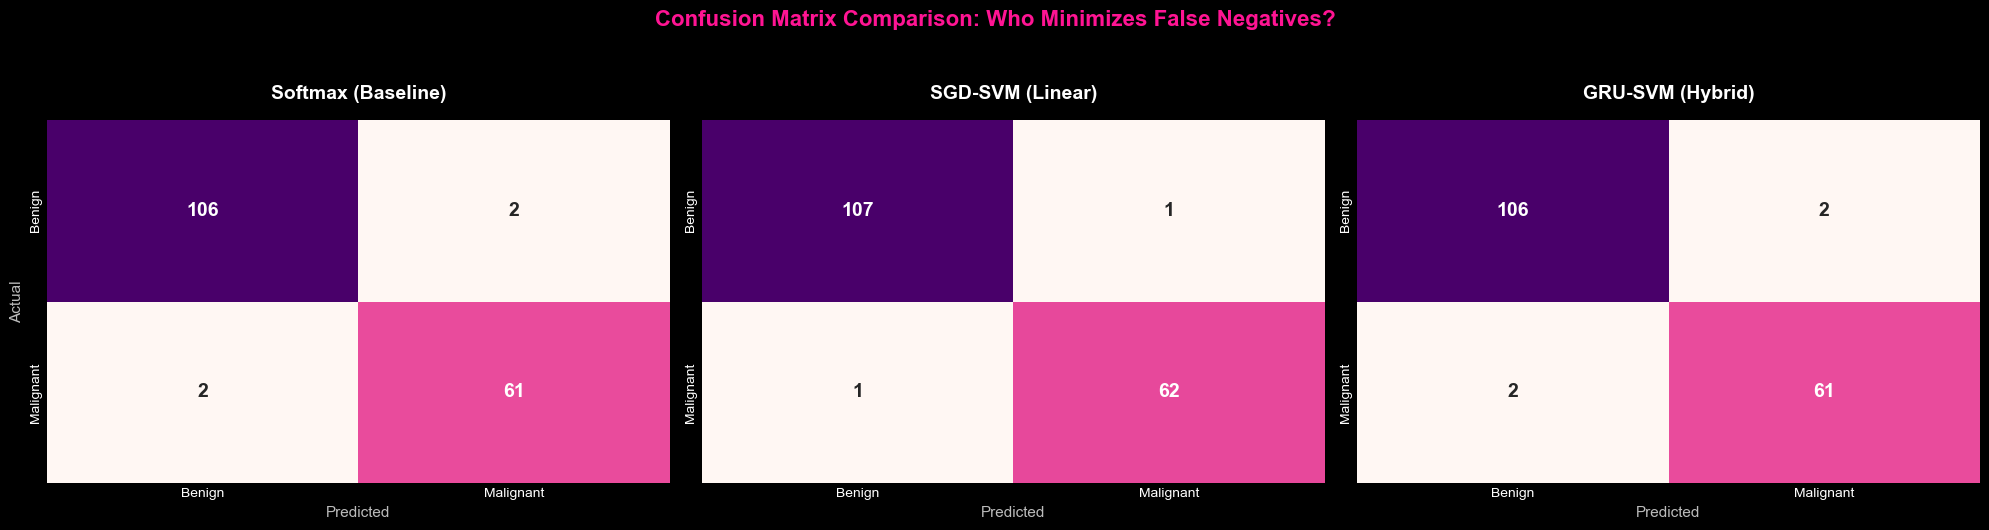
\includegraphics[width=0.9\textwidth]{images/confusion_bo1.png}
    \caption{Confusion Matrices for BO1 Models}
\end{figure}

\textbf{Interpretation:}
\begin{itemize}
    \item \textbf{SGD-SVM:} Demonstrates superior performance with only 1 False Negative, making it the safest model for clinical deployment.
    \item \textbf{Softmax:} Performs well with high sensitivity, missing only 2 cases.
    \item \textbf{GRU-SVM:} Shows competitive performance with the baseline, achieving the same sensitivity and low false negative rate (2), confirming the viability of the hybrid approach.
\end{itemize}

\subsection{ROC Curve Evaluation}
The Receiver Operating Characteristic (ROC) curves illustrate the diagnostic ability of the models.

\begin{figure}[H]
    \centering
    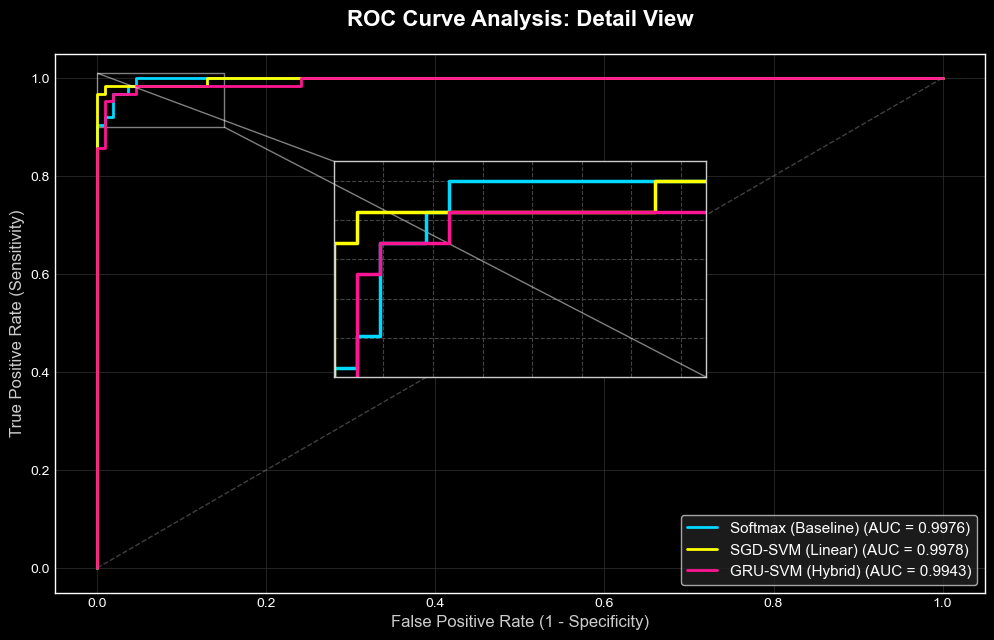
\includegraphics[width=0.8\textwidth]{images/roc_curve.png}
    \caption{ROC Curve Analysis}
\end{figure}

\subsection{Winning Model Selection}
Based on the comprehensive evaluation, \textbf{SGD-SVM (Linear)} is selected as the winning model for the Tumor Classification task.

\textbf{Rationale:}
\begin{itemize}
    \item \textbf{Medical Safety (Lowest FN):} It achieved the lowest number of False Negatives (1), meeting the strict safety requirements for a triage tool.
    \item \textbf{Accuracy Dominance:} It outperformed both the baseline and the hybrid model in overall accuracy (98.83\%).
    \item \textbf{Simplicity \& Robustness:} As a linear model, it is less prone to overfitting on this dataset size compared to the more complex GRU-SVM, leading to better generalization.
\end{itemize}

\section{BO2: Risk Triage (Stratification)}
The evaluation of the BO2 Risk Triage model focuses on the calibration quality of the predicted probabilities, ensuring that the risk scores correspond to actual event frequencies.

\subsection{Calibration Quality}
The SGD-SVM model was calibrated using Platt scaling (sigmoid calibration) to transform the decision function outputs into well-calibrated probabilities. The calibration quality was assessed using the Brier score and a reliability diagram.

The model achieved a Brier score of \textbf{0.0439}, indicating a high degree of calibration accuracy (where 0 represents perfect calibration). This low score confirms that the predicted probabilities are reliable estimates of the true risk.

\begin{figure}[h]
    \centering
    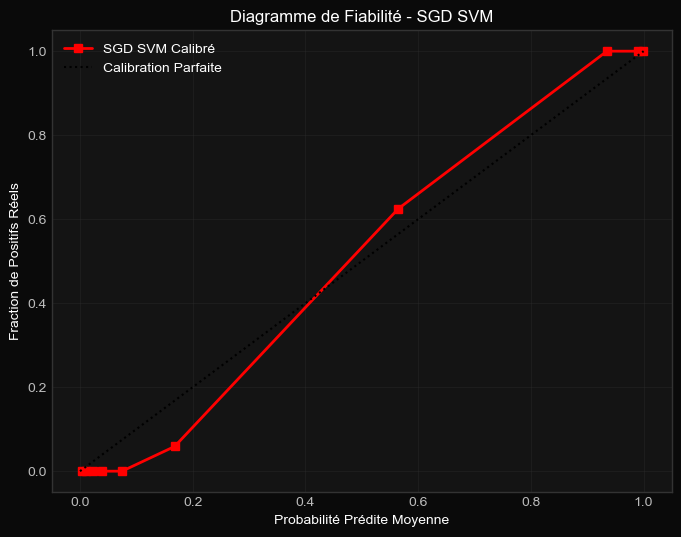
\includegraphics[width=0.8\textwidth]{images/calibration.png}
    \caption{Calibration Curve (Reliability Diagram) for the SGD-SVM Model. The plot shows the relationship between mean predicted probability and the fraction of positives (actual risk). The proximity of the curve to the diagonal dashed line indicates good calibration.}
    \label{fig:bo2_calibration}
\end{figure}

\section{Prognosis Model Results (BO3)}
For the prognosis task, we compared two ensemble methods: \textbf{Random Forest} (Bagging) and \textbf{Gradient Boosting} (Boosting).



\subsection{Comparative Performance Analysis}
The table below summarizes the performance of both models across the three target variables.

\begin{table}[H]
    \centering
    \caption{Performance Comparison: Random Forest vs. Gradient Boosting}
    \begin{tabular}{l|cc|cc|c}
        \toprule
        & \multicolumn{2}{c|}{\textbf{Aggressiveness}} & \multicolumn{2}{c|}{\textbf{Growth Rate}} & \textbf{Evolution 6M} \\
        \textbf{Model} & \textbf{$R^2$ Test} & \textbf{MAE Test} & \textbf{$R^2$ Test} & \textbf{MAE Test} & \textbf{Accuracy} \\
        \midrule
        Random Forest & 0.9963 & 0.0169 & 0.9905 & 0.2747 & \textbf{99.48\%} \\
        \textbf{Gradient Boosting} & \textbf{0.9986} & \textbf{0.0110} & \textbf{0.9962} & \textbf{0.1791} & 99.21\% \\
        \bottomrule
    \end{tabular}
\end{table}

\begin{figure}[H]
    \centering
    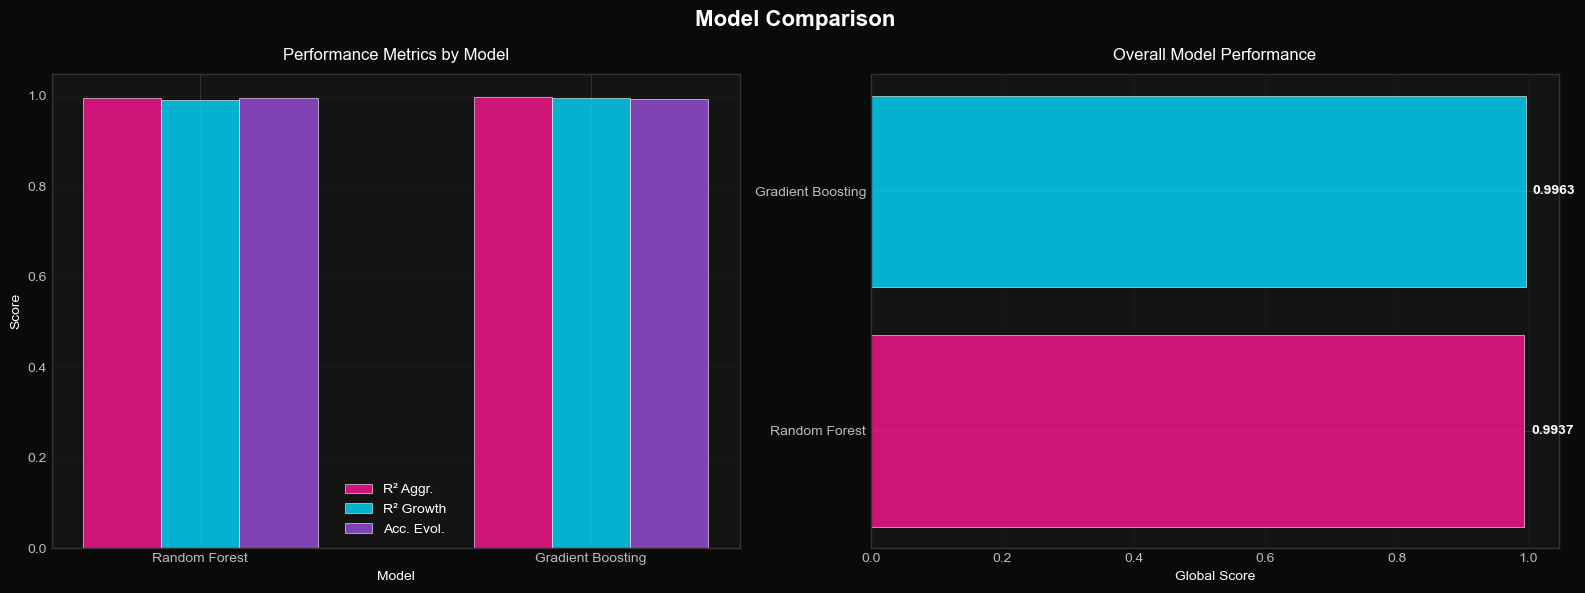
\includegraphics[width=0.9\textwidth]{images/meta_comp.png}
    \caption{Model Comparison: Metrics Overview}
\end{figure}

\subsection{Winning Model Selection}
\textbf{Gradient Boosting} is selected as the champion model. Although Random Forest achieved a marginally higher accuracy for the classification task (Evolution 6M), Gradient Boosting demonstrated superior precision in the regression tasks (Aggressiveness and Growth Rate), which are critical for detailed prognosis planning.

\subsection{Detailed Performance: Gradient Boosting}

\subsubsection{Predictions vs. Actuals}
The scatter plots below illustrate the alignment between predicted and actual values for the regression targets.

\begin{figure}[H]
    \centering
    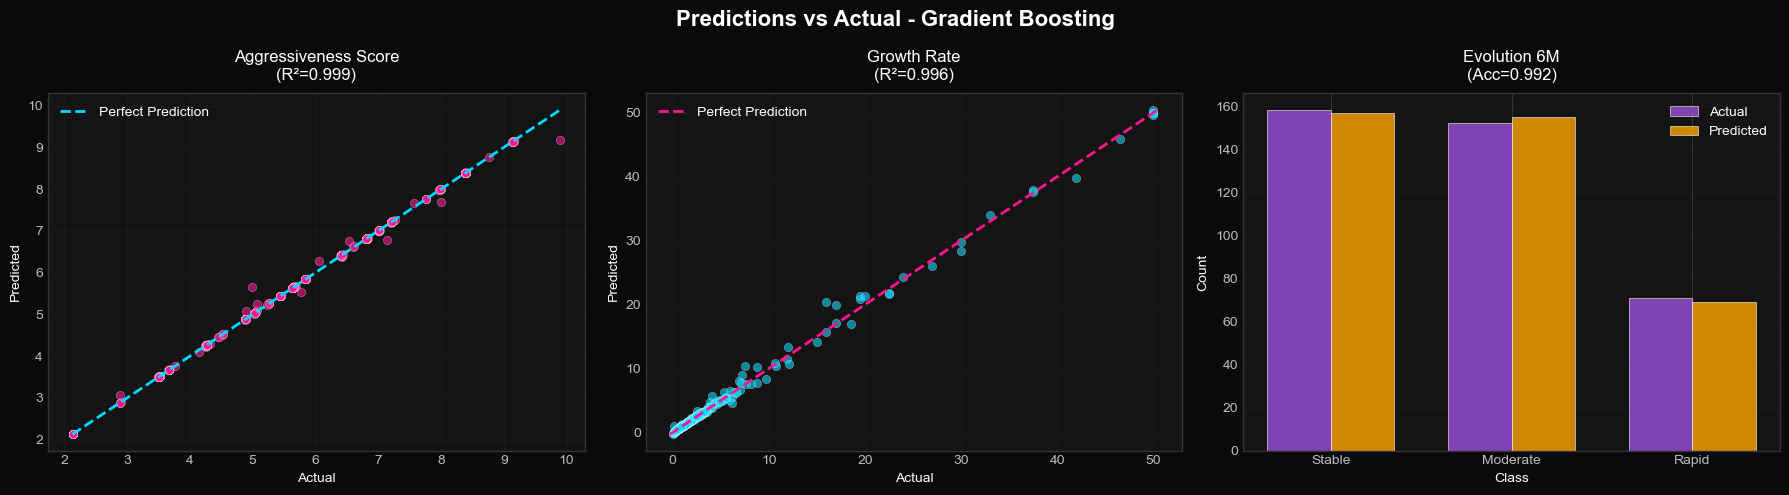
\includegraphics[width=0.9\textwidth]{images/predictionsvs.png}
    \caption{Predictions vs. Actual Values (Gradient Boosting)}
\end{figure}

\subsubsection{Confusion Matrix (Evolution 6M)}
The confusion matrix evaluates the classification performance for the 6-month evolution prediction.

\begin{figure}[H]
    \centering
    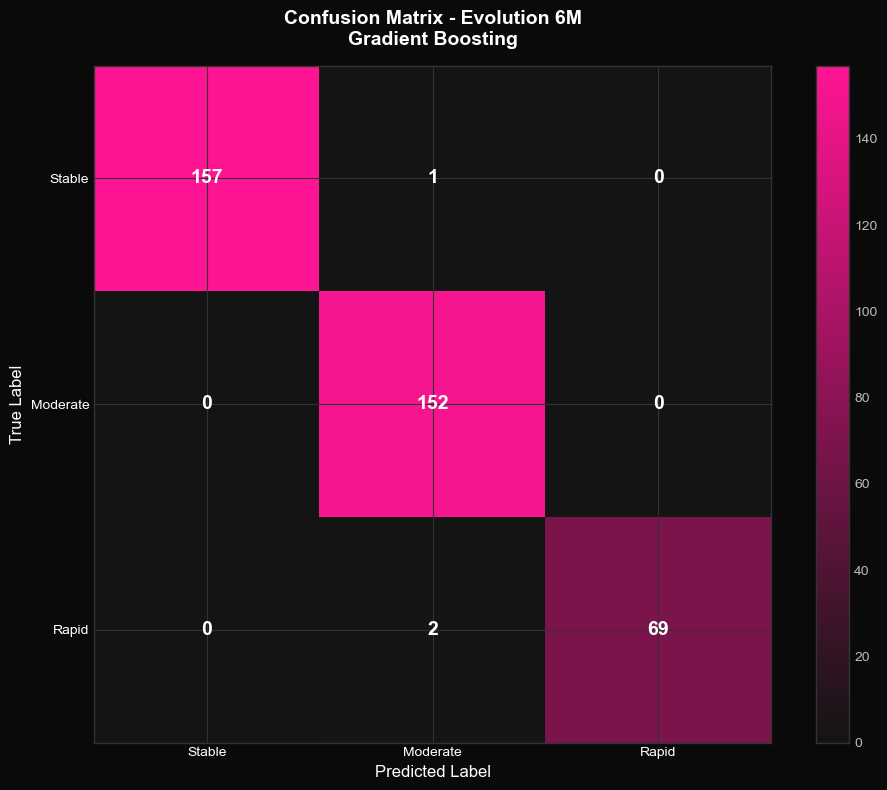
\includegraphics[width=0.7\textwidth]{images/conf_grad.png}
    \caption{Confusion Matrix: Evolution 6M (Gradient Boosting)}
\end{figure}

\textbf{Interpretation:} The model exhibits high diagonal density, indicating correct classifications across risk categories. Misclassifications are minimal, confirming the model's reliability for temporal risk assessment.

\subsubsection{ROC Curve Analysis}
The ROC curves for the multi-class evolution target demonstrate the model's discriminatory power.

\begin{figure}[H]
    \centering
    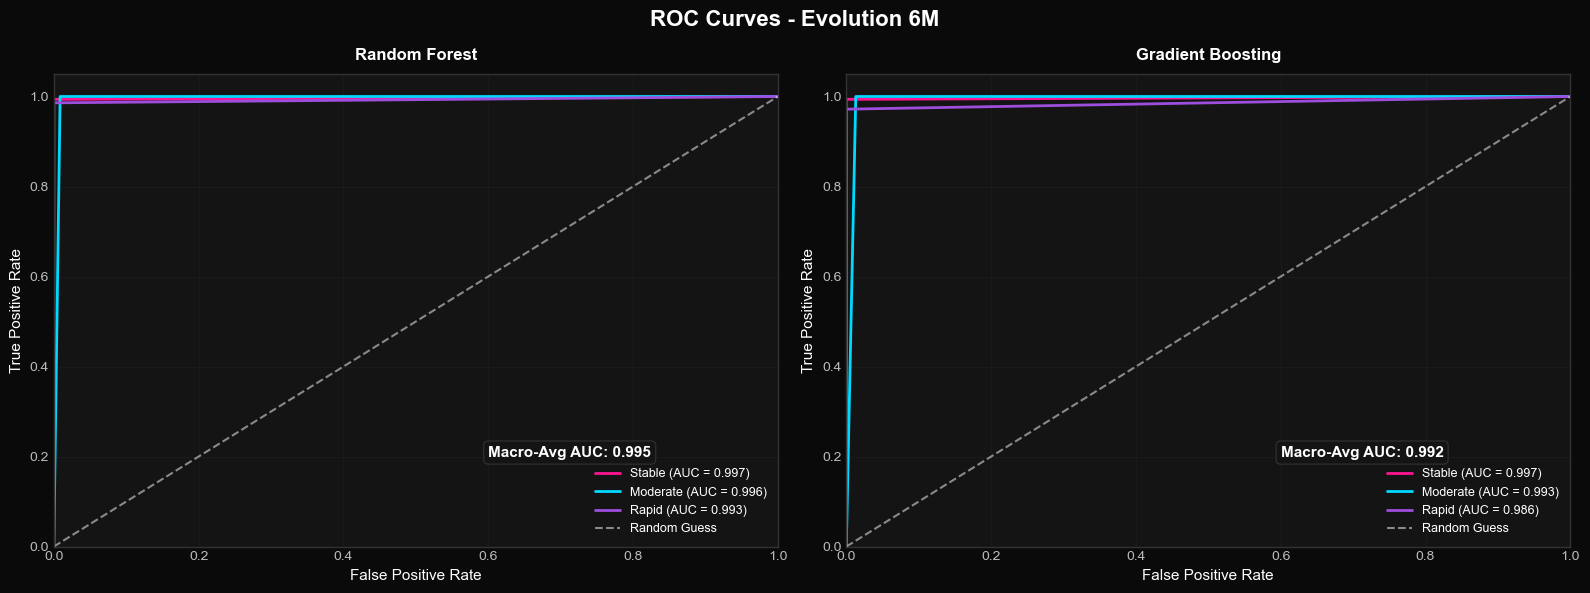
\includegraphics[width=0.8\textwidth]{images/roc_meta.png}
    \caption{ROC Curves for Evolution 6M}
\end{figure}

\subsubsection{Residual Analysis}
The residual plots check for homoscedasticity and bias in the regression predictions.

\begin{figure}[H]
    \centering
    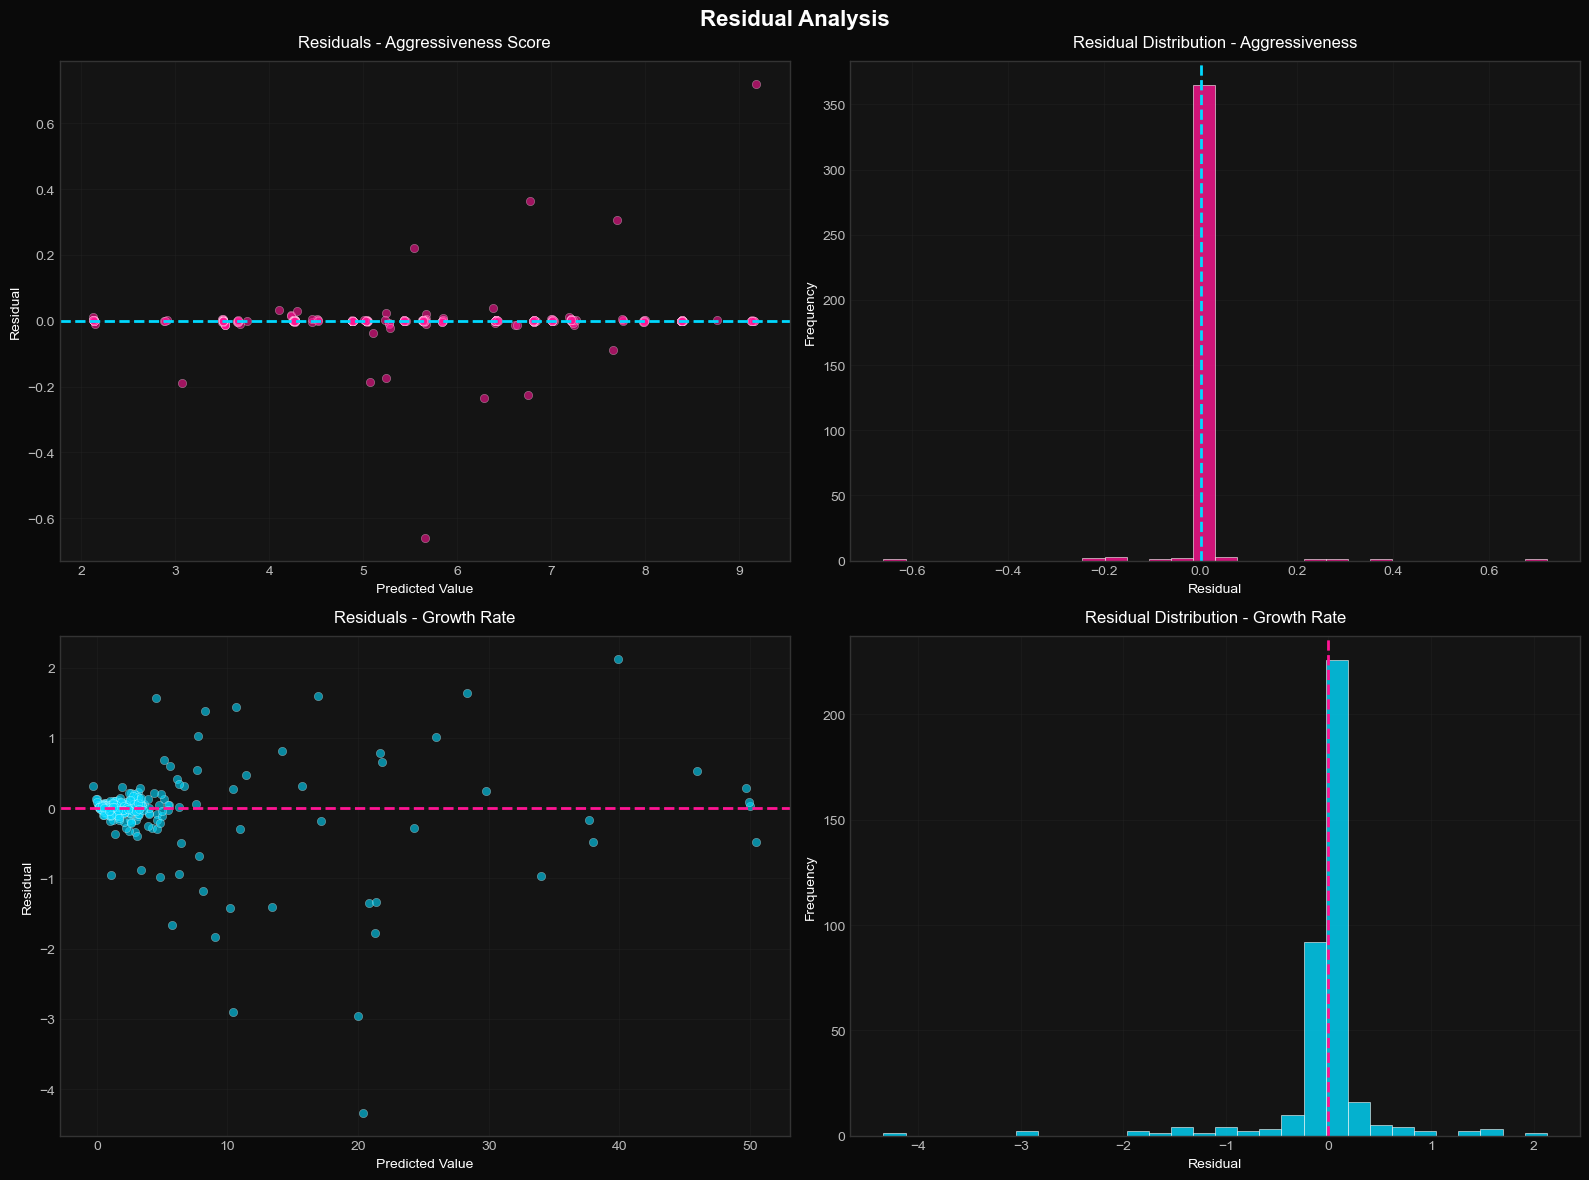
\includegraphics[width=0.9\textwidth]{images/residuals.png}
    \caption{Residual Analysis for Aggressiveness and Growth Rate}
\end{figure}

\subsection{Key Findings}
\begin{itemize}
    \item \textbf{Superiority of Boosting:} Gradient Boosting achieved near-perfect $R^2$ (0.9986) on the Aggressiveness Score, indicating it successfully captured the composite logic used to generate this target.
    \item \textbf{Reliability:} With >99\% accuracy on the 6-month evolution classification, the model provides a reliable "second opinion" for oncologists planning treatment schedules.
\end{itemize}


